\documentclass{article}
\usepackage[T1]{fontenc}
\hyphenation{synthetic}
\usepackage{template/iclr2027_conference,times}
\usepackage{amsmath,amssymb,graphicx,booktabs,array,hyperref,url,placeins}
\hypersetup{colorlinks=true,citecolor=blue,urlcolor=blue,linkcolor=blue,pdfauthor={},pdftitle={Evaluating JEPA-Inspired Motion Representations through Geometry and Gait Asymmetry}}
\newcommand{\dg}{^{\circ}}
\newcommand{\E}{\mathbb{E}}
\newcommand{\sg}{\operatorname{sg}}
\newcommand{\mean}{\operatorname{mean}}
\newcommand{\figurefile}[3]{\begin{figure}[t]\centering\includegraphics[width=\linewidth]{figures/#1.pdf}\caption{#2}\label{#3}\end{figure}}
\title{Evaluating JEPA-Inspired Motion\\
Representations through Geometry\\
and Gait Asymmetry}
\author{Anonymous authors}
\begin{document}
\maketitle
\begin{abstract}
We study whether motion representations inspired by joint-embedding predictive architectures (JEPA) preserve gait asymmetry when restoring complete windows of noisy 2D poses. Our adaptation of ideas from self-supervised learning uses paired synthetic motions and clean projected training references. Evaluation uses 14 development participants and three random training seeds. The main outcome is absolute error in recovering the change in knee-motion asymmetry between an original motion and its edited counterpart. A baseline that always predicts no change has mean error 5.81$\dg$, lower than all 16 trained variants with fixed penalties for failed measurements. Its error is 1.73$\dg$ lower than a model trained directly on joint coordinates (95\% interval [0.53, 3.15]$\dg$), although that model improves the noisy poses. The variant trained to predict differences between paired feature vectors has 0.37$\dg$ lower mean error than the variant predicting each vector separately. The 95\% interval [$-1.11$, 1.76]$\dg$ includes zero, leaving their relative accuracy uncertain. Adding training penalties for asymmetry-change errors and very short predicted limb segments increases mean knee-angle trajectory error in all eight model families. Giving less weight to the change penalty reduces trajectory error in the follow-up study. A post hoc geometric check finds more left--right assignment failures for the feature-difference variant despite its lower response-error estimate. These comparisons inform the evaluation of JEPA-inspired representations for future gait world models by testing measurement accuracy and geometric left--right assignment.
\end{abstract}

\section{Introduction}
Human gait offers a way to test whether learned representations preserve meaningful movement differences. A knee angle depends on the positions of the hip, knee, and ankle, while comparing the legs also requires knowing which joints belong to each side. Because the legs alternate during walking, symmetry cannot be assessed by expecting identical poses at every instant. Clinical studies illustrate why different measurements matter. After stroke, more symmetric step lengths can coexist with asymmetric joint mechanics \citep{padmanabhan2020symmetry}. In Parkinson's disease, gait asymmetry need not identify the clinically more affected side \citep{seuthe2024laterality}. In knee osteoarthritis, the relationship between pain and biomechanical asymmetry differs with unilateral versus bilateral symptoms \citep{creaby2012gait}. A model could therefore obscure useful movement differences by smoothing them away or assigning them to the other leg; greater symmetry alone does not establish healthier gait.

Self-supervised learning derives training targets from the data rather than requiring manual task labels. In a joint-embedding predictive architecture (JEPA), an encoder converts the observed context into feature vectors, and a predictor estimates the features of a target \citep{assran2023ijepa,bardes2024vjepa}. A feature vector is a learned numerical description of the input. Hierarchical JEPA has been proposed as part of world models that predict how a physical state changes, potentially in response to an action \citep{lecun2022path}. Applying this idea to gait requires checking whether features retain the movement differences needed downstream. Accurate feature prediction alone does not establish accurate knee trajectories or left--right assignment.

We study this question through controlled pose restoration. The student encoder receives estimated 2D joint positions, while a teacher encoder receives clean projected references during training. A decoder, called the readout, converts the student's features back into joint coordinates and is trained against those references. This uses paired synthetic supervision inspired by self-supervised learning. It restores an observed motion window; future-state prediction is outside the completed evaluation. We compare each original motion with a version containing a synthetic knee edit. The response measures how the left--right difference in knee-motion range changes between them. Physical mirroring, occlusion, and input naming swaps let us examine movement changes separately from observation errors.

We first ask whether predicting masked reference features improves response accuracy. The uncertain result motivates comparing two added objectives: matching each motion's features or their paired difference. When training for the response worsens knee-angle trajectories, a follow-up varies the readout objective while retaining the learned encoders. A later geometric check asks whether lower response error also means more reliable left--right assignment. Appendix~\ref{app:journey} summarizes the completed experimental sequence and the scope of its follow-up analyses. All stages reuse the development people, so follow-up analyses provide no independent confirmation.

\section{Related representation and restoration methods}
The closest skeletal precedent, S-JEPA \citep{abdelfattah2024sjepa}, predicts masked skeletal features and evaluates action recognition; General Feature Prediction also learns targets for masked skeleton modeling \citep{sun2025gfp}. Our adaptation supplies privileged projected references to the teacher and deploys the student for coordinate restoration, whereas S-JEPA uses its target encoder downstream. This comparison addresses measurement fidelity under that adaptation, without reproducing its recognition benchmark.

PoseBERT learns temporal 3D modeling through masking and denoising \citep{baradel2022posebert}; MotionBERT reconstructs 3D motion from noisy, partial 2D observations \citep{zhu2023motionbert}; SmoothNet refines temporal pose estimates to reduce jitter \citep{zeng2022smoothnet}. These methods motivate reconstruction and refinement controls, but their published tasks do not resolve our paired, side-sensitive response question. None was fitted as an external baseline here. Our comparisons concern the implemented procedures and their supervision, with claims limited accordingly.

\section{Paired movement restoration}
\subsection{States, projected targets, and anatomical names}
Let $M_a$ be a complete body-model motion window and $M_b=\mathcal E_\delta(M_a)$ its edited counterpart. We apply the nominal right-knee edit $\delta\in\{0,5,10,15\}\dg$ before optional physical mirroring $T_m$. A fixed camera $c$ then gives reference coordinates $Y_i=\pi_c(T_mM_i)$ for each state $i\in\{a,b\}$. Rendering and pose estimation, with occlusion and naming corruption, produce observed coordinates $X_i$ with confidence, availability, and timestamps. Each pair shares its camera, physical orientation, and observation conditions. Corruption and restoration retain the $128\times12\times2$ coordinate array, joint-slot order, and timestamps. Masks mark missing values without deleting slots, and the model predicts $\widehat Y_i$ on the same grid. The array shape stays fixed while the synthetic edit changes its geometry.

For anatomical leg $\ell\in\{L,R\}$, let $\theta_{i,\ell,t}$ be the image-plane angle between the knee-to-hip and knee-to-ankle vectors. We summarize its range of motion by subtracting the 5th from the 95th percentile, then compare the legs and the paired states:
\begin{equation}
q_{i,\ell}=P_{95}(\theta_{i,\ell})-P_5(\theta_{i,\ell}),\qquad
A_i=q_{i,R}-q_{i,L},\qquad \Delta A=A_b-A_a.
\label{eq:measurement}
\end{equation}
Thus $q$ measures knee-angle excursion, $A$ is right-minus-left asymmetry, and $\Delta A$ is the change in that asymmetry between paired motions. It is not a time derivative and does not by itself identify which leg changed. We recompute targets after projection because the nominal 3D edit need not equal the image-plane response.

\figurefile{method}{Experimental workflow, with illustrative keypoints showing a synthetic 3D knee edit. Endpoint and delta learn from noisy poses and clean projected references in separate runs, then fit a reference-supervised readout. Equation~\ref{eq:feature} defines the feature losses. Each development window is restored independently. Paired outputs and references determine asymmetry-change error; knee-angle trajectories and post hoc naming are scored per window. The development cohort is reused across studies. This diagram shows the frozen-encoder procedures; direct fitting jointly trains encoder and readout.}{fig:method}

Exchanging the computed excursions $(q_L,q_R)$ reverses the sign of $A=q_R-q_L$. Physical mirroring instead reflects the 3D body, exchanges its side indices, and projects it through the same camera. Projection need not exchange the excursions exactly, so we do not assume that this operation reverses the response's sign. A naming swap changes only the estimated input, including confidence and availability; reference names stay fixed. The restoration task must therefore correct the naming error while preserving the intended movement change.

\subsection{Representations, readouts, and comparison logic}
Each model token groups four consecutive frames of one joint, giving 384 tokens in a transformer that can use the full observed window. Tokens retain joint and time identifiers even when coordinates are masked. The student predicts the reference features of a slowly updated teacher using cross-entropy \citep{caron2021dino}. VICReg discourages constant or redundant features \citep{bardes2022vicreg}. Translation and scale are computed only from available observations that were not artificially masked. We apply this same normalization to the references, so reference geometry and hidden coordinates cannot influence its statistics. Appendices~\ref{app:integrity} and~\ref{app:methods} give the tensor layout and training specification.

We compare two additional feature losses. The endpoint loss matches predicted and reference features separately for each motion; the delta loss matches their difference across the pair. For a token queried in both motions, $p_i$ and $t_i$ are the predictor and teacher scores before softmax (logits). With teacher center $c$ and channel-mean removal $H$, define
\begin{equation}
e_i=H[p_i/0.1-\sg\{(t_i-c)/0.06\}],\quad
L_{E,k}=\frac{\|e_a\|^2+\|e_b\|^2}{2D},\quad
L_{\Delta,k}=\frac{\|e_b-e_a\|^2}{2D}.
\label{eq:feature}
\end{equation}
Here $\sg$ stops gradients through the teacher. We average valid common queries within each pair, then give pairs equal weight. Both losses supplement the base feature objective with the same training-calibrated coefficient. Shared errors in $e_a$ and $e_b$ can cancel in the delta loss, so improving it need not improve either motion separately. The teachers also evolve separately, and the two losses initially exert unequal influence on training (Section~\ref{sec:feature}).

\begin{table}[t]\centering\small
\caption{Three questions organize the completed experiments. Each row shows the primary comparison recorded for that study. ``Change'' combines coordinate, scalar-response, and geometry losses. These stages reuse the same development people; they are not independent replications.}
\label{tab:design}
\setlength{\tabcolsep}{3pt}
\begin{tabular}{>{\raggedright\arraybackslash}p{1.36in}>{\raggedright\arraybackslash}p{1.78in}>{\raggedright\arraybackslash}p{2.04in}}\toprule
Question & Candidate versus comparator & What the comparison measures \\\midrule
Does feature prediction help? & Core JEPA versus direct fitting; both use change supervision & Pooled response error. JEPA freezes its encoder; direct fitting adapts it. \\
Does predicting feature differences help? & Delta versus endpoint JEPA; both use change supervision & Pooled response error. Both encoders are frozen; the added pretraining target differs. \\
Does denser readout supervision help? & Dense angular change versus low scalar weight, using the same delta encoder & ViTPose waveform error. Only readout training changes; the encoder stays fixed. \\\bottomrule
\end{tabular}
\end{table}

Zero response and unchanged observations establish task baselines; direct coordinate fitting measures practical restoration. Initialized, shuffled-reference, and coordinate-pretrained encoders test what information pretraining contributes. Figure~\ref{fig:restoration} retains every fitted configuration for the shared waveform check; Appendix~\ref{app:inventory} summarizes the primary contrasts without treating configurations as independent evidence.

The readout predicts coordinate corrections at observed joints and absolute coordinates at missing joints. Encoders are frozen (held fixed) except in direct fitting, which trains encoder and readout together. Coordinate supervision minimizes $L_x$. The original ``change'' objective adds two penalties: $L_s=\E[((\Delta\widehat A-\Delta A)/180)^2]$ for response error, and $L_g$ for predicted segments shorter than two pixels where references admit measurement. Comparing $L_x+L_s+L_g$ with $L_x$ cannot separate their effects. The follow-up holds coordinate and geometry supervision fixed. It compares a lower response weight, $L_x+0.1L_s+L_g$, with $L_x+\lambda_dL_d+L_g$, where $L_d$ measures squared error in paired angular changes at each valid leg and timestamp, divided by $180^2$. Training-only batches set its initial gradient magnitude to match the low-scalar term. Appendix~\ref{app:methods} specifies the reductions and updates.

\subsection{Data, outcomes, and inferential scope}
We select walking candidates from AMASS motion capture \citep{mahmood2019amass}; Appendix~\ref{app:methods} describes screening. Before constructing motion variants, the dataset split assigns each recorded person to training, development, or locked confirmation. Every derived motion and corrupted variant keeps that assignment. Fitting uses 112 training people, 692 motions, and 1,645 windows; evaluation uses 14 different development people and 155 windows, including 12 people from BioMotionLab\_NTroje and two from KIT. No independent confirmation test was completed. We resample motion to 25 Hz and form 128-timestamp windows before creating paired variants. These transformations change the raw data while preserving the fixed model-input shape.

The design crosses two cameras, original/mirrored states, clear/occluded images, three naming conditions, and RTMPose-M, HRNet-W32, and ViTPose-base estimates \citep{jiang2023rtmpose,sun2019hrnet,xu2022vitpose}. ViTPose and the 15$\dg$ edit are excluded from optimization and calibration, while rendering-derived boxes remove person-detector uncertainty. Training and coefficient calibration select training-person pairs only. Development targets may be read for data-integrity checks, but do not supply optimization losses; fitting excludes locked-confirmation data. These controls separate fitting from development scoring, while repeated inspection of development results still informs later design choices.

For each primary comparison, let $G$ be comparator error minus candidate error; positive values favor the candidate. The initial no-benefit null is $H_0:\E[G]\leq0$ for core JEPA versus direct fitting with the change objective. The next comparison tests delta versus endpoint with that objective; the follow-up tests dense versus low-scalar ViTPose waveform error for delta. This notation retrospectively describes the recorded comparisons, retaining their two-sided intervals without a new one-sided test. ``Declared'' means documented in the study records, not preregistered. All stages reuse seeds 17, 29, and 43 and the development cohort. Coordinate-only contrasts are secondary. The naming checks, stratified analyses, failure-cost sensitivity, and new figure intervals are exploratory, without adjustment for multiple comparisons. Appendix~\ref{app:inventory} summarizes the three primary questions and their paired effects.

Response error is $|\Delta\widehat A-\Delta A|$ in degrees. Waveform error measures the average absolute error in the knee-angle trajectory over both legs and reference-valid timestamps. Coordinate error (NLE) divides joint distance by the rendered person-box diagonal. Lower values are better for all three. Angular evaluation requires at least 16 valid frames and 80\% coverage on reference support shared across variants of a source window. Nonfinite predictions or predicted segments shorter than two pixels count as failures, scored at 180$\dg$ for waveforms and 720$\dg$ for responses. The naming check uses different eligibility rules (Section~\ref{sec:naming}). The zero-response baseline always predicts $\Delta\widehat A=0$; it produces no restored trajectory.

We average conditions within windows, windows within motions, and motions within people, then average over seeds. Extra renderings therefore do not count as additional people. For the core and response studies, 2,000 bootstrap draws resample people and seeds separately while keeping methods paired; we call these crossed intervals. The readout-repair study first averages each person's paired differences over seeds, then uses a Student-$t$ interval across 14 people. This person-$t$ interval is conditional on the three fitted seeds. Appendix~\ref{app:evaluation} details the weighting and interval calculations.

\section{Results: what supports faithful restoration?}
\subsection{Coordinate restoration helps, but pooled response recovery is limited}
\label{sec:restoration}
Direct coordinate training improves response error from 12.69$\dg$ for unchanged observations to 7.54$\dg$, waveform error from 18.57$\dg$ to 12.07$\dg$, and NLE from 0.0718 to 0.0298. Its exploratory paired response gain is 5.14$\dg$ [2.15, 8.65]$\dg$ (crossed 95\% interval). Every person's seed-averaged waveform and coordinate errors improve, while response error improves for 10 of 14 people. Appendix Figure~\ref{fig:cases} shows all 14 people, including those whose response worsens, and separates clear from occluded observations. These participant-level summaries show paired errors; reconstructed pose examples are unavailable.

\figurefile{restoration}{Restoration quality and supervision tradeoffs. A--B: all eight families and both objectives, as hierarchical means over 14 people and three seeds, pooled over estimators. Circles use coordinate supervision; open triangles add scalar and geometry terms. Direct fitting adapts its encoder; all other encoders are frozen. Zero response (5.81$\dg$) appears only in A. C: paired change-minus-coordinate waveform effects with crossed-person/seed 95\% intervals (2,000 draws), newly computed and exploratory; positive values indicate deterioration. Responses and waveforms retain failures at 720$\dg$ and 180$\dg$, respectively. Families share the development cohort and are not independent replications.}{fig:restoration}

The zero-response baseline predicts $\Delta\widehat A=0$ for every pair, giving error $|\Delta A|$. Its pooled mean is 5.811$\dg$, below all 16 neural variants under the original scoring rule. It estimates no movement change: its low error reflects the cost of always returning zero relative to the models' estimated responses and occasional measurement failures. Small true responses favor this baseline, while invalid reconstructions incur the large failure cost. Thus improving noisy poses does not, in this evaluation, establish better recovery of asymmetry changes than zero prediction. The result concerns these pooled scores, not whether the models contain any response information.

Separating results by visibility and edit level helps explain the pooled comparison (Table~\ref{tab:strata}); this analysis is exploratory. Direct coordinate training beats zero response in both clear-image edit groups, but not in either occluded group. The endpoint and delta variants with change-trained readouts have higher error than zero prediction in all four groups. The 5/10$\dg$ and 15$\dg$ labels are nominal edit levels, not bins of true projected response. The available aggregate results omit per-pair true magnitudes; binning already averaged signed responses would not recover that analysis. We report every selected observation-by-edit group and retain all observation-by-estimator groups and all 16 methods in the technical supplement (Appendix~\ref{app:strata}).

\begin{table}[t]\centering\small
\caption{Exploratory response errors by observation and nominal edit, in degrees. Direct uses coordinate supervision and joint fitting; endpoint and delta use frozen encoders with the original change readout. All groups contain the same 14 people and three seeds. The last column is a paired zero-minus-direct effect with crossed 95\% interval; positive favors direct. Original 720$\dg$ failure scoring is retained.}
\label{tab:strata}
\setlength{\tabcolsep}{3.5pt}\begin{tabular}{lrrrrl}\toprule
Observation, edit & Zero & Direct & Endpt. & Delta & Zero $-$ direct [95\% CI]\\\midrule
Clear, 5/10$^\circ$ & 4.10 & 2.79 & 4.54 & 4.33 & 1.32 [1.22, 1.42] \\
Clear, 15$^\circ$ & 9.23 & 6.12 & 9.95 & 9.64 & 3.10 [2.88, 3.30] \\
Occluded, 5/10$^\circ$ & 4.10 & 9.54 & 12.65 & 12.08 & -5.44 [-8.31, -3.03] \\
Occluded, 15$^\circ$ & 9.23 & 14.49 & 17.82 & 17.47 & -5.26 [-8.33, -2.73] \\
\bottomrule\end{tabular}

\end{table}

\subsection{The incremental feature-prediction benefit remains unresolved}
\label{sec:feature}
With the original change readout, mean response error is 9.99$\dg$ for delta and 10.36$\dg$ for endpoint. The 0.37$\dg$ difference favors delta, but its crossed 95\% interval [$-1.11$, 1.76]$\dg$ includes both worse and better performance. Coordinate-only readouts reverse the point estimates: delta has error 10.94$\dg$ and endpoint 10.23$\dg$. However, the estimated effect of changing the readout on this comparison is also uncertain: 1.09$\dg$ [$-0.65$, 2.85]$\dg$. These results establish neither a delta benefit nor a reliable dependence on readout choice. The earlier core-JEPA advantage over direct fitting is 0.69$\dg$ [$-0.64$, 1.98]$\dg$. Both use the change objective; this primary comparison does not use the stronger direct-coordinate model.

The two added feature losses also differ in their initial influence on training. The shared coefficient $\lambda_J=0.0126468$ was calibrated on 32 training batches so that the larger auxiliary parameter gradient had a root-mean-square magnitude 10\% of the base objective's gradient. This gives endpoint 10\%, but delta only 0.0013\%, before clipping. Across the six new delta/endpoint pretraining fits, the total gradient was clipped to norm one on 11,999 of 12,000 updates. Calibration records and training logs verify these values (Appendix~\ref{app:optimization}). They show that equal coefficients did not give equal initial gradient influence. They do not establish whether that imbalance persisted or caused the final ranking, so the comparison applies to these fitted procedures rather than JEPA in general.

\subsection{Rare failures materially affect the response contrast}
\label{sec:failure}
With $F$ denoting a failed eligible response and $w$ the hierarchical population weights, the score at cost $C$ is
\begin{equation}
S(C)=\underbrace{\E_w[\mathbf1_{\neg F}|\Delta\widehat A-\Delta A|]}_{U\text{: unconditional successful contribution}}
+C\Pr_w(F).
\label{eq:cost}
\end{equation}
At the original $C=720\dg$, endpoint and delta fail on 0.563\% and 0.525\% of the weighted population. The corresponding failure penalties contribute 4.055$\dg$ and 3.778$\dg$ to their mean scores; valid outputs contribute 6.306$\dg$ and 6.210$\dg$. Failure penalties therefore account for 0.277$\dg$, or approximately 74\%, of the 0.373$\dg$ difference between means. This percentage describes part of the score difference, not the frequency or cause of failures. Averaging error only over successful outputs requires dividing their contribution by their population share: $U/(1-\Pr_w(F))$ (Appendix~\ref{app:cost}).

\figurefile{reliability}{Reliability and uncertainty have different denominators. A: descriptive person-balanced response failure percentages for three fitted procedures. B: unconditional successful-error and 720$\dg$ failure-cost contributions, whose sum is the response score. Bars are not conditional success-only errors. C: paired endpoint-minus-delta response effects at four fixed costs, with crossed-person/seed 95\% intervals over 14 people and three seeds; positive favors delta. The filled point retains the declared 720$\dg$ comparison. Costs 360$\dg$ and 180$\dg$ are exploratory stress tests; zero is an accounting lower bound assigning failures no error. All four intervals cross zero. Methods in A--B are grouped by their named supervision, not matched encoder adaptation.}{fig:reliability}

Valid responses can differ by at most 720$\dg$, the original failure cost. Exploratory rescoring at 0, 180, 360, and 720$\dg$ gives delta advantages of 0.10, 0.17, 0.23, and 0.37$\dg$, all with intervals spanning zero (Figure~\ref{fig:reliability}). Appendix~\ref{app:cost} explains these scales and locates the complete cost inventory; no cost is selected as preferable. In particular, both predictive variants' successful contributions already exceed 5.811$\dg$: neither can beat zero response at any nonnegative failure cost with these predictions and weights. Their pooled deficit therefore cannot be attributed to the failure penalty alone. This lower-bound argument assigns failures zero error; it is not a success-only comparison.

\subsection{Readout weighting substantially changes waveform fidelity}
\label{sec:repair}
Adding the response and geometry penalties to coordinate supervision increases mean waveform error in all eight model families (Figure~\ref{fig:restoration}). In the five core families, the increase also appears in every person's seed-averaged score and every seed's population mean. For core JEPA, response error falls from 10.69$\dg$ to 10.07$\dg$, while waveform error rises from 17.45$\dg$ to 22.55$\dg$. Training for the scalar response can therefore accompany less accurate knee-angle trajectories. Because this comparison adds two penalties together, it does not identify which one causes the deterioration.

\figurefile{repair}{Readout repair on ViTPose. A--B: waveform means and person-$t$ 95\% intervals after averaging three seeds within each of 14 people. The direct-coordinate row is jointly trained; the three repair rows share a frozen encoder. C--D: paired comparator-minus-candidate waveform gains using the same person-$t$ procedure, positive favoring the first named arm. Delta dense versus low scalar is the declared primary; endpoint is secondary. Other displayed intervals are exploratory and unadjusted, and are conditional on the three fitted seeds. All waveform scores include 180$\dg$ failures. Marginal intervals in A--B do not substitute for paired contrasts in C--D.}{fig:repair}

The follow-up keeps the delta and endpoint encoders fixed and varies readout supervision while retaining the coordinate and geometry terms (Figure~\ref{fig:repair}). For delta on ViTPose inputs, waveform error is 23.17$\dg$ with the original objective, 19.47$\dg$ with low scalar weight, and 19.19$\dg$ with dense supervision. Lowering scalar weight improves this error by 3.70$\dg$ [2.58, 4.81]$\dg$ (exploratory paired-person interval). Dense supervision adds an uncertain 0.28$\dg$ improvement over low scalar weight: the declared interval is [$-0.19$, 0.75]$\dg$, and the crossed-bootstrap sensitivity interval is [$-0.44$, 0.86]$\dg$. Its response gain is 0.13$\dg$ [$-2.69$, 2.94]$\dg$. This interval supports neither better response accuracy nor a claim that response accuracy is preserved.

For the endpoint encoder, the secondary dense-versus-low-scalar waveform gain is 0.72$\dg$ [0.39, 1.05]$\dg$, without adjustment for multiple comparisons. Both dense variants still have about six degrees more error than direct coordinate fitting on ViTPose. The low-scalar change accounts for 93\% of delta's mean improvement from the original to the dense objective. This ratio summarizes the means; it does not explain why they differ. The dense angular term changes where its gradients act and what they target. The study therefore supports sensitivity to loss weighting, while leaving the proposed mechanism involving sparse percentile gradients untested.

\FloatBarrier
\subsection{Response ranking does not establish anatomical naming fidelity}
\label{sec:naming}
We examined left--right assignment after the response results. The check uses reference-valid hip, knee, and ankle pairs separated by at least four pixels. Let $d_n,d_s$ be summed Euclidean distances with the predicted names retained or exchanged. Assignment fails if exchanging names improves error by more than two pixels, if the two errors differ by at most two pixels (ambiguous), or if predictions are nonfinite (missing). These eligibility rules differ from the angular checks. The recorded rates combine these failures, so their separate rates cannot be verified; 50\% is not an established chance baseline.

\figurefile{laterality}{Post hoc geometric assignment diagnostic. Points show failure means for every naming condition; intervals are exploratory crossed-person/seed 95\% intervals over 14 people and three seeds. Each estimates its method mean, not a pairwise effect. Failure combines wrong, ambiguous, and missing predictions on separately eligible bilateral hip/knee/ankle pairs. Endpoint strata retain the executed 4:1 nonheld/held weighting. All estimators, cameras, physical orientations, and observation conditions are pooled. Direct uses joint coordinate fitting; endpoint and delta use frozen encoders and the original change readout. No categorical lines or chance baseline are implied.}{fig:laterality}

Under global naming swaps, assignment failure reaches 81.12\% for endpoint and 83.40\% for delta, compared with 23.29\% for direct coordinate fitting (Figure~\ref{fig:laterality}). The pooled delta rate is 50.46\%, versus endpoint's 49.69\%, despite delta's lower response-error point estimate. The exploratory excess is 0.77 percentage points [0.17, 1.53] (crossed 95\% interval), unadjusted and not a replacement for the response primary. Direct's left/right excursion errors are 17.94/17.19$\dg$, versus delta's 15.70/15.29$\dg$, including 180$\dg$ failure costs. The delta outputs have lower per-leg excursion errors but more frequent geometric assignment failures than the direct-coordinate outputs.

\FloatBarrier
\section{Discussion and limitations}
Self-supervised learning with JEPA motivates asking whether predictable features preserve useful movement measurements. In this study, direct coordinate training improves noisy poses, yet always predicting zero gives lower pooled response error. These outcomes concern different tasks: restoring trajectories and recovering the change in asymmetry between paired motions. Geometric checks further show that the lower delta response-error estimate accompanies more assignment failures than endpoint. The incremental JEPA benefit remains uncertain.

The contrast between physical mirroring and naming errors matters because plausible geometry can still be assigned to the wrong leg. Clinical use therefore requires separate validation of anatomical identity and the chosen gait measure. Our synthetic knee edits do not reproduce disease or treatment response, and their asymmetry scores have no established diagnostic interpretation.

The intervals for the initial JEPA and later feature-difference comparisons both span zero, leaving their benefits uncertain. Interpretation is limited by unequal initial gradient influence and fixed training budgets, alongside separately evolving teachers and a small readout. Direct fitting also updates its encoder and receives different coordinate-supervised exposure. The follow-up more clearly supports the importance of scalar-loss weighting than an additional benefit from dense supervision. Neither initialization diagnostics nor decomposing the final score establishes what caused the fitted predictions.

The same 14 development people and three fitted seeds inform successive design choices. Person-disjoint fitting and fixed indexing reduce leakage risks, but no locked-person confirmation, GAVD evaluation, or natural-video study provides an independent test. Synthetic preparation further limits clinical interpretation. Biomechanical validation would require independent anatomical measurements, as in OpenCap's comparison with laboratory references \citep{uhlrich2023opencap}. The available results support reaggregation and participant-level summaries, but lack the complete reconstructed poses and checkpoints needed to repeat the full pipeline.

A next study should fix its response, waveform, and naming comparisons before inspecting new people, match auxiliary influence across JEPA variants, and retain zero-response and jointly trained controls. Developing gait world models would additionally require explicit future-state or action-conditioned prediction, followed by testing on natural observations with synchronized anatomical references.

\label{maintextend}
\clearpage
\section*{AI use disclosure}
The human authors originated the research ideas and wrote the initial manuscript drafts. They reviewed the AI-assisted revisions, made the final edits, verified the full text, reported results, and references, and approved the final manuscript. The human authors take full responsibility for its content and conclusions.

Under the authors' direction, AI assistants helped refine and critique the scientific framing, inspect research code, analysis materials, and recorded experimental results, analyze results, identify and check literature and submission requirements, draft and revise text, and create analysis, plotting, and document-build code. Assistant reviews also checked methods, numerical summaries, figures, and page layouts. These supporting checks were followed by the human authors' final verification and approval. No new study models were trained or participant data collected during this manuscript revision.
\bibliography{references}
\bibliographystyle{template/iclr2027_conference}
\clearpage
\appendix
\section{Data integrity and evaluation}
\label{app:integrity}
\label{app:evaluation}
The study fits models on 112 people (692 motions, 1,645 windows) and evaluates them on 14 different development people (155 windows). Every edit, mirror, view, and corrupted observation inherits its source person's split. Known duplicate motion hashes cannot cross splits. Training excludes the 15$\dg$ edit and ViTPose inputs. Their evaluation still uses the same development people; no locked-person confirmation was completed.

\begin{figure}[h]\centering
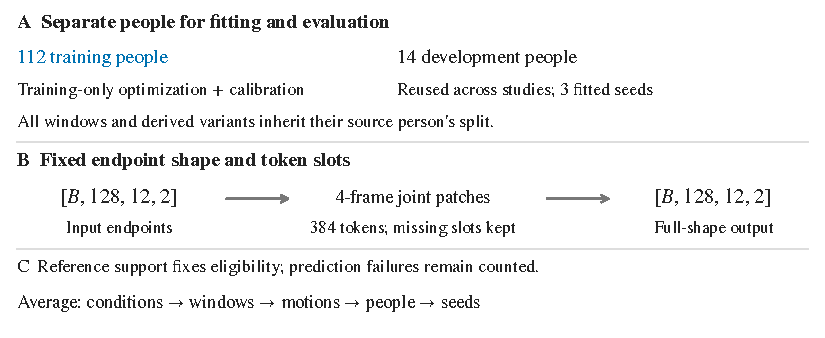
\includegraphics[width=\linewidth]{figures/protocol.pdf}
\caption{Data preparation and evaluation protocol. Source-person identity determines the split before variants are created. Four-frame patches regroup the fixed joint/time array without dropping missing slots. Fitting and loss calibration use training pairs; evaluation retains reference-eligible failures and averages repeated observations before people. The development cohort is reused across all stages.}
\label{fig:protocol}
\end{figure}

\paragraph{What stays fixed.} Preparation resamples motion to 25 Hz, selects nonoverlapping windows, and creates synthetic observations; it changes values and record counts. The model preserves the resulting $[B,128,12,2]$ coordinate layout, with confidence and availability $[B,128,12]$ and timestamps $[B,128]$. Each token packs four frames of one joint; decoding restores their original positions. Neither leg is separately time-warped or rescaled. Input naming swaps permute observations and their confidence/availability together while reference anatomy stays fixed.

\paragraph{What fitting can access.} Student inputs contain observed coordinates, native confidence, availability, and time. Projected references supply training targets and teacher inputs. Origin and isotropic scale use available, artificially unmasked observations only; references share that transform. Optimization and gradient calibration use training pairs. Data-integrity checks may read development references for consistency and identity, but these references do not enter fitting losses. Locked-confirmation participants are excluded from fitting. Unknown person aliases and overlap with pose estimators' training data remain possible.

\paragraph{What counts in evaluation.} Reference support is shared across variants of each source window. Angular scoring requires finite reference geometry, segments at least two pixels long, at least 16 frames, and 80\% coverage. Prediction failures remain eligible and receive the declared costs. Means average conditions within windows, windows within motions, motions within people, then seeds. Nonheld/held groups retain 2:1 response weighting and 4:1 endpoint weighting; extra renderings do not increase the participant count.

\paragraph{How uncertainty is calculated.} Core and feature-response comparisons use 2,000 paired bootstrap draws (RNG seed 731), independently resampling 14 people and three seeds. Repair first averages each person's differences over seeds, then uses $\bar d\pm t_{.975,13}s_d/\sqrt{14}$; its crossed bootstrap is a sensitivity check. This person-$t$ interval conditions on the fitted seeds. Neither procedure accounts for adaptive reuse of development results.

\clearpage
\section{Reproducible training specification}
\label{app:methods}
\label{app:optimization}
The full technical supplement retains loss reductions, masking rules, and optimizer equations. The specifications below identify the fitted procedures and the controls needed to interpret them. Recorded experimental configurations and training logs establish the completed settings.

\paragraph{Observations and geometry.} Walking candidates are screened from AMASS filenames and projected geometry, without clinical verification. Right-knee edits of 0, 5, 10, or 15 degrees are gated by an ankle-height proxy and taper at window boundaries. Editing precedes physical mirroring. Cameras, fitted across each window's original, edited, and mirrored motions, remain fixed; oblique and side views use 45 and 90 degrees. References are projected body-model joints, including image-hidden joints. Nominal 3D edit angles need not equal projected response changes.

\paragraph{Model and masking.} Five channels per frame (two coordinates, confidence, availability, time) give a 20-dimensional joint patch, mapped to width 96. The encoder has four layers and four heads; the predictor has two layers. Joint and time identifiers persist through masking. Graph--time masks hide connected joint regions and time intervals, using about half the available tokens while retaining context. Unavailable slots remain in the 384-token sequence. The readout uses LayerNorm, a $96\to96$ linear map, GELU, and a zero-initialized $96\to8$ map. It adds coordinate corrections where observed and predicts absolute coordinates where missing.

\paragraph{Losses and support.} Coordinate fitting averages squared normalized error over reference-valid coordinates, then endpoints equally. The base feature objective uses centered teacher--student cross-entropy (temperatures 0.06/0.1) plus $0.05L_{\rm VICReg}$; it follows the DINO mechanism rather than I-JEPA's regression. VICReg uses translated views with invariance/variance/covariance weights 25/25/1. Endpoint and delta auxiliaries (Equation~\ref{eq:feature}) average common queries within pairs, then pairs equally; all four reference frames must be valid in both patches. Shuffled-reference pretraining instead uses another window of the same person, preserving observation conditions and endpoint role.

The original readout minimizes $L_x+L_s+L_g$, low scalar uses $L_x+0.1L_s+L_g$, and dense uses $L_x+\lambda_dL_d+L_g$. Both angular terms use squared errors divided by $180^2$. Dense supervision averages the squared error between predicted and reference paired angle changes over common supported legs and timestamps. Geometry loss penalizes predicted segments shorter than two pixels on reference-defined support. Thus the original coordinate-to-change comparison adds two penalties together. Repair keeps geometry and coordinate terms fixed.

\paragraph{Updates and calibration.} Seeds are 17, 29, and 43. Pretraining and frozen readout fitting each use 2,000 updates; direct fitting uses 4,000 joint updates. Batch size is 16; draws sample person, motion, window, then pair uniformly at each level. AdamW uses peak rate $3\times10^{-4}$, 5\% warmup, cosine decay, weight decay 0.01, and gradient-norm clipping at one. Teacher momentum rises from 0.99 to 0.999; the center momentum is 0.9. Fresh readouts share initialization across arms (seed $+100003$). Equal update totals do not match encoder adaptation or supervised exposure.

On 32 training batches at seed-17 initialization, the shared feature coefficient $\lambda_J=0.0126468$ gives endpoint gradients 10\% of base RMS magnitude and delta 0.001303714\%, before clipping. The six new feature fits clip 11,999 of 12,000 updates. For each repair encoder/seed, 32 training batches instead calibrate $\lambda_d$ to low scalar's initial gradient magnitude. These records describe initialization and clipping; they do not establish later influence, convergence, or the cause of a ranking.

\clearpage
\section{Primary questions and supporting comparisons}
\label{app:inventory}
Each primary comparison estimates a paired difference in measurement error between two fitted procedures. Figure~\ref{fig:questions} summarizes the three declared primary contrasts. For each, gain is comparator error minus candidate error after the recorded averaging. A retrospective no-benefit null is $H_{0,j}:\mu_j\leq0$, against $\mu_j>0$. We retain two-sided 95\% intervals; this notation implies neither preregistration nor a new one-sided test.

\begin{figure}[h]\centering
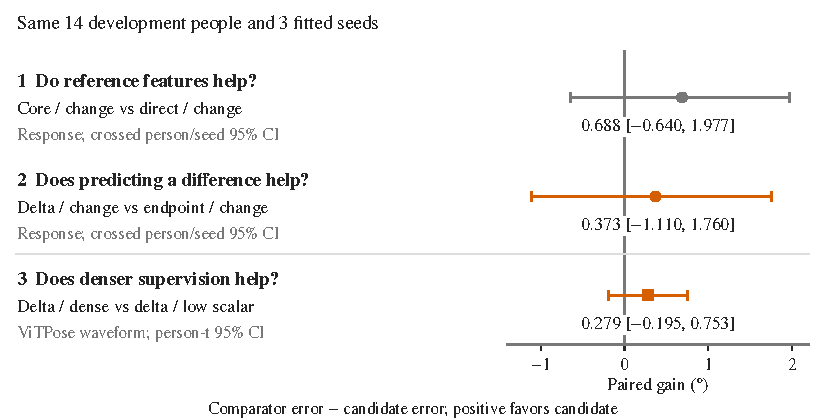
\includegraphics[width=\linewidth]{figures/study-questions.pdf}
\caption{Three sequential questions, with their recorded primary gains and 95\% intervals. The first two concern pooled response error and use crossed person/seed bootstraps. The third concerns ViTPose waveform error and uses a person-$t$ interval after seed averaging. Positive values favor the candidate. Different outcomes and inference procedures are separated; there is no pooled effect. Every interval spans zero, leaving each primary benefit unresolved. All comparisons reuse 14 development people and three fitted seeds.}
\label{fig:questions}
\end{figure}

\paragraph{Baselines establish the scale.} Zero response has pooled error 5.81$\dg$ and supplies no trajectory or anatomical assignment. Unchanged observations score 12.69$\dg$ response and 18.57$\dg$ waveform error; direct coordinate fitting improves these to 7.54$\dg$ and 12.07$\dg$. The initial primary instead compares core JEPA with direct fitting under the original change objective. Replacing its comparator with direct coordinate fitting would change the question.

\paragraph{Controls constrain the feature claim.} Figure~\ref{fig:restoration} retains all eight encoders/training procedures with both readout objectives, including initialized features, shuffled references, and coordinate pretraining. These controls ask whether useful information comes from fitting a readout, preserving correspondence, or reconstructing coordinates. They are diagnostic variants within one cohort. The complete means remain in the technical supplement; no configurations are averaged into a new method.

\paragraph{Follow-ups change the interpretation.} Under coordinate-only readouts, delta has higher response error than endpoint (10.94$\dg$ versus 10.23$\dg$), reversing their ordering under the original change objective. The interaction remains uncertain. Adding the original change package increases waveform means in all eight procedures, by 4.39--7.21$\dg$. On ViTPose, lowering delta's scalar weight improves waveform error by 3.70$\dg$ [2.58, 4.81]$\dg$; the smaller additional dense-supervision benefit is the third primary above. Reduced waveform error does not establish preserved response accuracy. These exploratory comparisons explain the next question without supplying independent confirmation.

\clearpage
\section{Diagnostics and reproducibility}
\label{app:strata}
\label{app:cost}
\label{app:failures}
\label{app:repair}
\label{app:reproduction}
\label{app:journey}
\paragraph{Observation conditions.} Main Table~\ref{tab:strata} shows every clear/occluded by nominal-edit group for the task baselines and the focal direct, endpoint, and delta procedures. Direct coordinate fitting beats zero response in both clear-image groups and neither occluded group; endpoint and delta with change readouts exceed zero in all four. The supplement retains all 16 variants in all four groups and all six visibility-by-estimator groups. The 5/10$\dg$ versus 15$\dg$ distinction describes nominal edits, not bins of true projected response. The available aggregate results omit the per-pair values required for that latter analysis.

\paragraph{Failure costs and denominators.} For $\theta\in[0,180]\dg$, excursion lies in $[0,180]\dg$, signed asymmetry in $[-180,180]\dg$, and paired response in $[-360,360]\dg$. The maximum discrepancy between valid responses is therefore 720$\dg$, the original failure cost. Waveform failures cost 180$\dg$. Equation~\ref{eq:cost} keeps failed cases in the population. If $U$ is the unconditional successful-error contribution and $f$ the weighted failure fraction, $U/(1-f)$ is a conditional error; adding it to failure cost would mix denominators.

Figure~\ref{fig:reliability} retains every examined cost (0, 180, 360, 720$\dg$). The endpoint-minus-delta gain ranges from 0.10$\dg$ to 0.37$\dg$, with every interval spanning zero. At zero cost, failures remain with zero error. Endpoint and delta's successful contributions, 6.31$\dg$ and 6.21$\dg$, already exceed zero response's 5.81$\dg$, so changing to any nonnegative cost cannot reverse that comparison with predictions and weights fixed. This argument does not apply automatically to other procedures.

\paragraph{Anatomical assignment.} The post hoc check uses reference-valid bilateral hip/knee/ankle pairs separated by at least four pixels. It compares named and swapped Euclidean errors with a two-pixel margin. Wrong, ambiguous, and nonfinite predictions all count as failures; only their combined rate is stored. This support differs from angular support, and 50\% is not an established chance level. Lower per-leg excursion error can coexist with more assignment failures (Figure~\ref{fig:laterality}); neither quantity verifies clinical identity or diagnosis.

\paragraph{Experimental sequence.} The first study compares reference-feature learning with direct fitting. The second tests whether matching paired feature differences improves response accuracy beyond matching each motion separately. Observed waveform deterioration motivates the third study, which varies readout supervision while retaining the encoders. Geometric assignment and the expanded sensitivity analyses follow inspection of these results. Alternative mask policies, learned external refiners, and movement re-pairing were not evaluated. All three studies reuse the development cohort, so this sequence supplies no independent confirmation.

\paragraph{Reproducibility scope.} The supplementary technical reference provides complete model and loss specifications, all configuration-level results, and the full condition and failure-cost analyses. Participant-level results support reaggregation and independent checks of the reported summaries. Repeating training additionally requires the motion and body-model assets, rendered observations, pose arrays, and complete checkpoints, which are not included in the available materials. No locked-confirmation or natural-video evaluation was completed.

\clearpage
\section{Participant profiles of response improvement and deterioration}
\label{app:cases}
Figure~\ref{fig:cases} shows every development person in the same order across panels. Direct coordinate restoration has lower seed-averaged response error than unchanged observations for 10 of 14 people. Relative to zero response, it has lower error for all 14 under clear images and for one under occlusion. The comparison shows lower response error than zero prediction under clear observations and higher error for most people under occlusion. Here improvement and deterioration refer to paired error differences; they are distinct from the binary measurement failures in Appendix~\ref{app:cost}. No clinical status is inferred from these profiles.

\begin{figure}[h]\centering
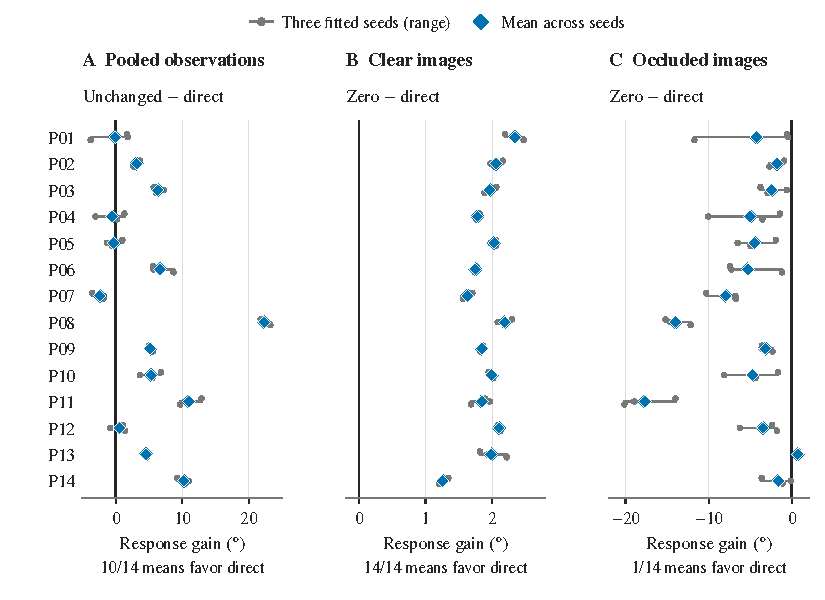
\includegraphics[width=\linewidth]{figures/cases.pdf}
\caption{Participant response profiles, with all 14 development people shown without selection. A: unchanged-minus-direct error, pooled over observations. B--C: zero-minus-direct error for clear and occluded images. Positive values favor jointly fitted direct coordinate restoration. Diamonds average seeds 17, 29, and 43; gray points and horizontal ranges show those fitted values, not confidence intervals. The original 720$\dg$ failure cost and hierarchical aggregation are retained; nonheld/held response strata have 2:1 weighting. Estimators, cameras, naming conditions and physical orientations are pooled. P01--P14 refer to the same people in every panel. Axis ranges differ. These exploratory summaries are not reconstructed poses or clinical examples.}
\label{fig:cases}
\end{figure}

\end{document}
